\documentclass[10pt,twocolumn]{article}
\usepackage[T1]{fontenc}
\usepackage{lmodern}
\usepackage[margin=0.72in,columnsep=0.24in]{geometry}
\usepackage{graphicx}
\usepackage{array}
\usepackage{hyperref}
\hypersetup{hidelinks,pdftitle={Where Modular Minecraft Agents Break}}
\setlength{\parindent}{0.95em}
\setlength{\parskip}{0pt}
\renewcommand{\arraystretch}{1.08}

\title{\textbf{Where Modular Minecraft Agents Break:}\\A Controlled Study of Deterministic Mechanics, Learned Visuomotor Specialists, and Frontier-Model Planning}
\author{Independent MineStudio Research Project}
\date{September 2026}

\begin{document}
\maketitle

\begin{abstract}
We evaluate a three-level Minecraft agent in which a frontier multimodal model performs planning (System~2), verified programs execute deterministic mechanics (System~0), and STEVE-1-derived policies control uncertain visual interaction (System~1). The decomposition yielded a real but narrow result: targeted behavior cloning increased paired stone-acquisition success from 37\% to 66\% (+29 percentage points; paired bootstrap 95\% CI $[+17,+41]$; exact McNemar $p=8.96\times10^{-6}$). However, seemingly safer System~0 handoffs reduced success from 66\% to 57\%, and targeted PPO reduced the champion from 66\% to 54\%. In a fresh-world iron-pickaxe study, none of three systems completed the objective. The full architecture reached a stone pickaxe in 15/22 valid runs and three raw iron in 2/22, but produced no ingots; vanilla System~1 with the same planner reached a stone pickaxe in 18/24 and raw iron in 1/24. The scripted no-System-2 arm never reached a stone pickaxe. The results support modular decomposition as a diagnostic and engineering tool, but not the stronger claim that the implemented architecture solves long-horizon Minecraft.
\end{abstract}

\section{Introduction}
Minecraft combines long-horizon planning, partial observability, navigation, continuous camera control, discrete inventory interfaces, and exact crafting dependencies. Video PreTraining (VPT) showed that large-scale video pretraining can produce a broad behavioral prior from native mouse and keyboard actions~\cite{vpt}. STEVE-1 added open-ended text conditioning to that prior~\cite{steve}. MineStudio exposed these models, simulation, fine-tuning, and benchmarking through a common environment API~\cite{minestudio}.

This project tested a systems hypothesis: high-level reasoning should be rented from an interchangeable frontier model; open-world motor competence should be inherited and selectively adapted; deterministic mechanics should be executed by verified programs. The practical question is empirical: \emph{does this decomposition improve complete tasks, or merely move errors between modules?}

The principal result is negative but informative. Local competence improved substantially without composing into long-horizon autonomy. Better imitation loss did not imply better behavior, removing deterministic errors did not guarantee higher system success, and verifier-driven PPO did not preserve the best behavioral checkpoint.

Our contributions are:
\begin{itemize}
  \item a paired behavioral selection protocol showing that the offline-loss winner was not the Minecraft-behavior winner;
  \item a System~0 library with explicit preconditions, success predicates, timeouts, aborts, and structured handoffs;
  \item seven randomized recovery micro-benchmarks separating an almost-solved skill from near-zero skills;
  \item a targeted PPO experiment that improved a development proxy but harmed frozen end-to-end hazard performance; and
  \item a long-horizon iron-pickaxe test that falsified the strong version of the architecture thesis in its current implementation.
\end{itemize}

\begin{figure}[t]
  \centering
  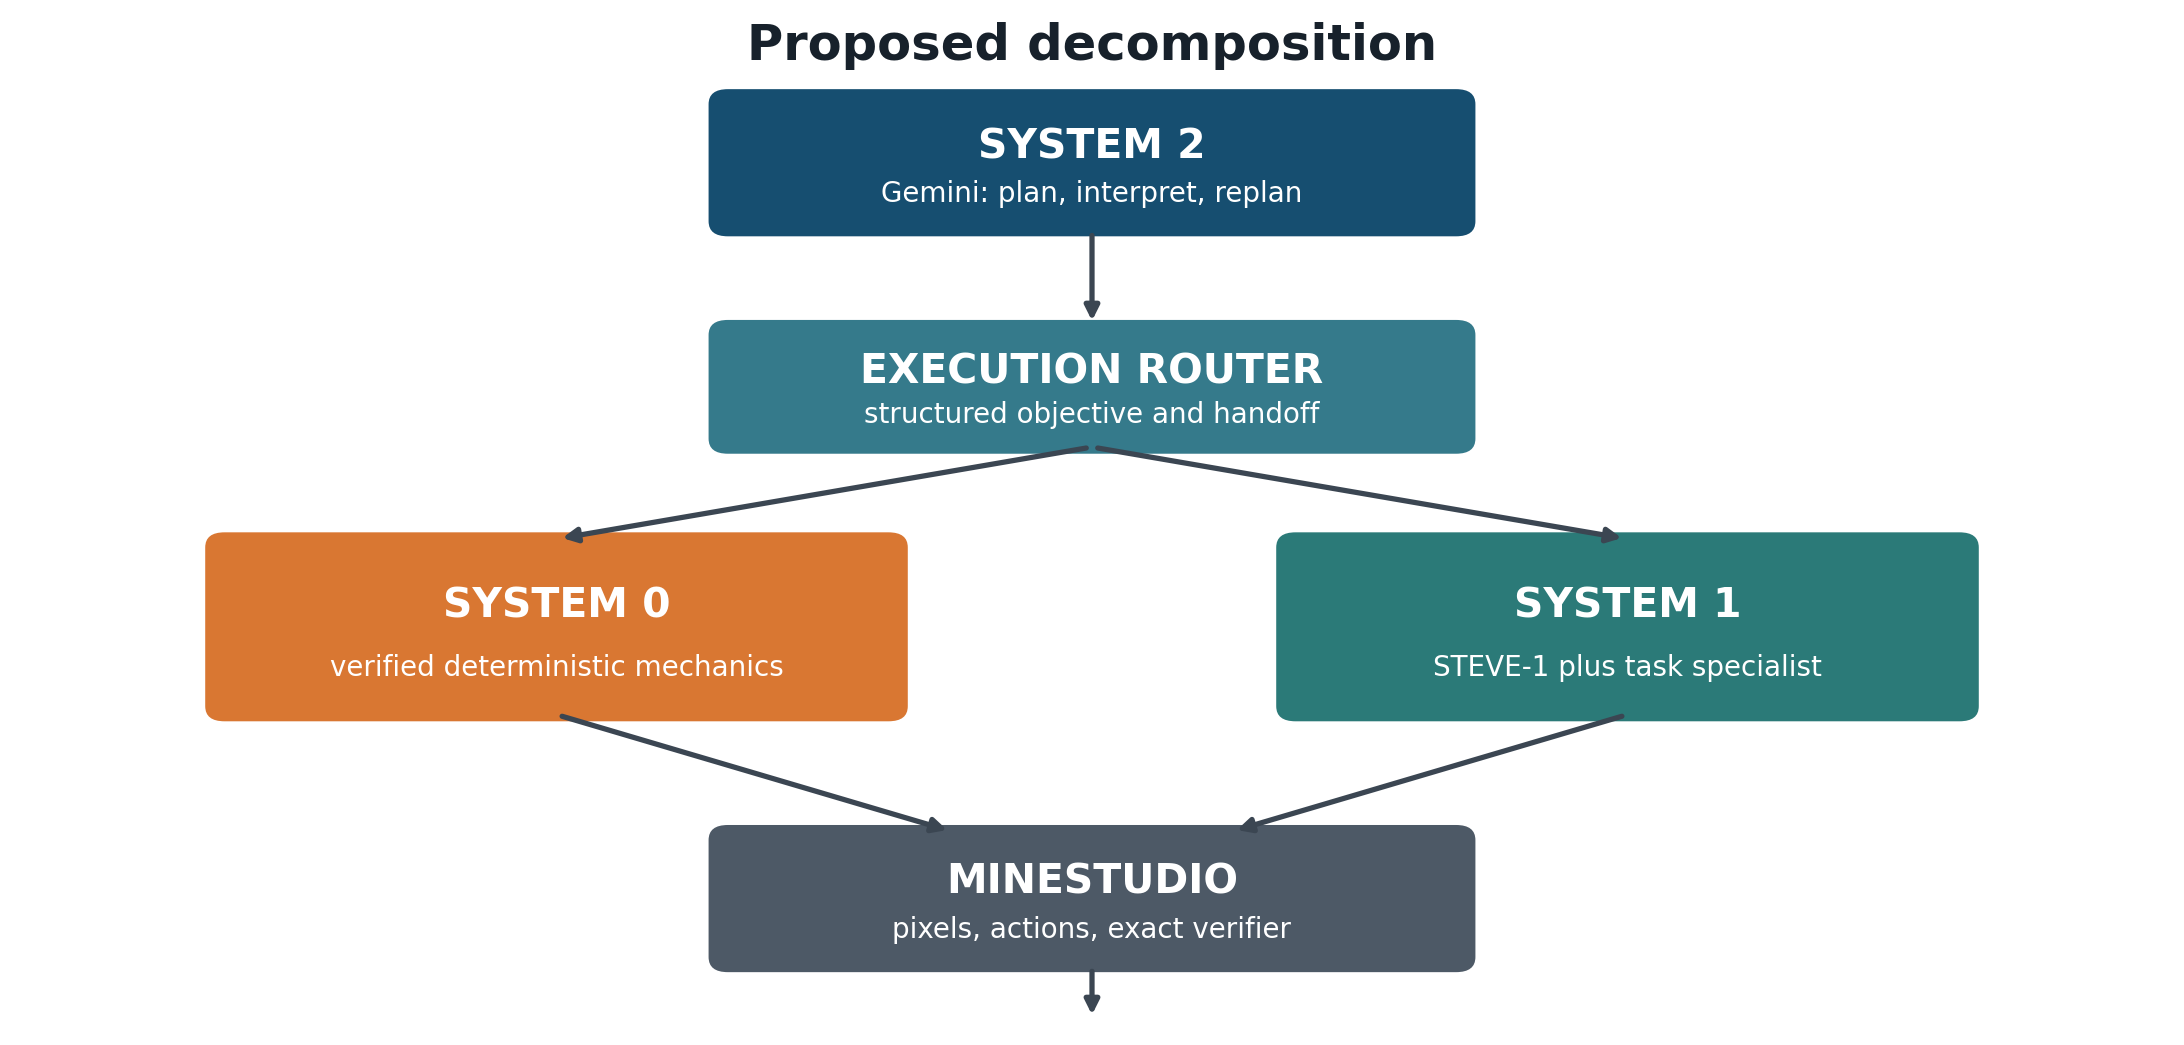
\includegraphics[width=\columnwidth]{figures/architecture.png}
  \caption{System~2 chooses objectives and replans; the router dispatches exact mechanics to System~0 and uncertain visual control to System~1; MineStudio supplies pixels, actions, events, and exact verification.}
  \label{fig:architecture}
\end{figure}

\section{Architecture}
\paragraph{System 2.}
Gemini 3.8 Flash received sampled frames and structured state, maintained the global objective, emitted a short-term objective and immediate instruction, interpreted failures, and replanned. No hidden map, resource coordinates, or world-state oracle was exposed.

\paragraph{System 1.}
Vanilla STEVE-1 handled general open-world behavior. The selected stone specialist was an upper-layer LoRA with rank 32, trained for acquisition and recovery. Routing invoked this specialist only for relevant stone/recovery instructions and vanilla STEVE-1 elsewhere.

\paragraph{System 0.}
Bounded action packets handled crafting, equipment, placement, station lifecycle, mining completion, pickup, and related mechanics. Every skill exposed preconditions, execution, success and failure predicates, timeout, abort conditions, and a structured result including \texttt{NEEDS\_SYSTEM1} when geometry became uncertain. Six initial skills passed live smoke tests and the contract/adapter suite passed 17 tests.

The boundary deliberately excluded open-ended search and hidden-map pathfinding. System~0 answered how to execute a known operation; System~1 handled uncertain perception and terrain; System~2 decided what to do and why.

\section{Experimental Design}
All direct policy comparisons used identical seeds and initial states. Success was defined from MineStudio state, not from language-model judgment. Gemini critiques were diagnostic labels, never numerical reward.

\begin{table}[t]
\centering
\caption{Experimental sequence.}
\label{tab:experiments}
\scriptsize
\begin{tabular}{@{}p{0.28\columnwidth}rp{0.48\columnwidth}@{}}
\hline
Experiment & Episodes & Question \\
\hline
Stage-0 baseline & 1000 & Where does pretrained execution fail? \\
Policy screen & 800 & Which BC checkpoint acts best? \\
System~0 isolation & 400 & Which boundary change caused regression? \\
Recovery micro-tests & 350 & Which System~1 skills are weakest? \\
Targeted PPO & 450 eval. & Can RL repair residual skills? \\
Iron-pickaxe viability & 70 valid & Does the full stack compose? \\
\hline
\end{tabular}
\end{table}

The final long-horizon run stopped at 70 valid episodes because of external API spending limits: the Full arm contains 22/24 valid seeds, while both controls contain 24/24. We report this incompleteness explicitly and make no final-success superiority claim.

\section{Results}
\subsection{A broad baseline hid a concentrated hazard failure}
Across a broad 1,000-episode distribution, the current STEVE-plus-options system acquired three cobblestone in 834 episodes (83.4\%; Wilson 95\% CI $[81.0,85.6]$). Aggregate success was misleading: water-near-stone success was 54.6\%, and swamp success was 69.0\%. Primary failures included 86 water-entry failures and 43 block-broken-without-collection failures.

This established a useful distinction. Pickup completion was a deterministic tail suitable for System~0; losing the target, terrain traps, and water recovery were learned-control problems.

\subsection{Targeted BC produced a strong narrow specialist}
Figure~\ref{fig:behavioral} shows the paired behavioral screen. Rank-32 upper LoRA at step 6400 achieved 75\% normal and 60\% hazard success, versus 47.5\% and 30\% for vanilla. Combined success rose from 37\% to 66\%. The +29-point effect had paired bootstrap 95\% CI $[+17,+41]$ and exact McNemar $p=8.96\times10^{-6}$. Water-conditioned success improved from 27.9\% to 58.2\%; post-water stone reacquisition improved from 32.4\% to 67.2\%.

The offline sweep selected rank-8 upper LoRA by validation loss (2.062), but rank-32 was the behavioral winner. Continuing rank-8 from 4800 to 6400 steps increased normal success while reducing hazard success from 53.3\% to 35.0\%. Behavioral checkpoint selection was therefore essential.

\begin{figure*}[t]
  \centering
  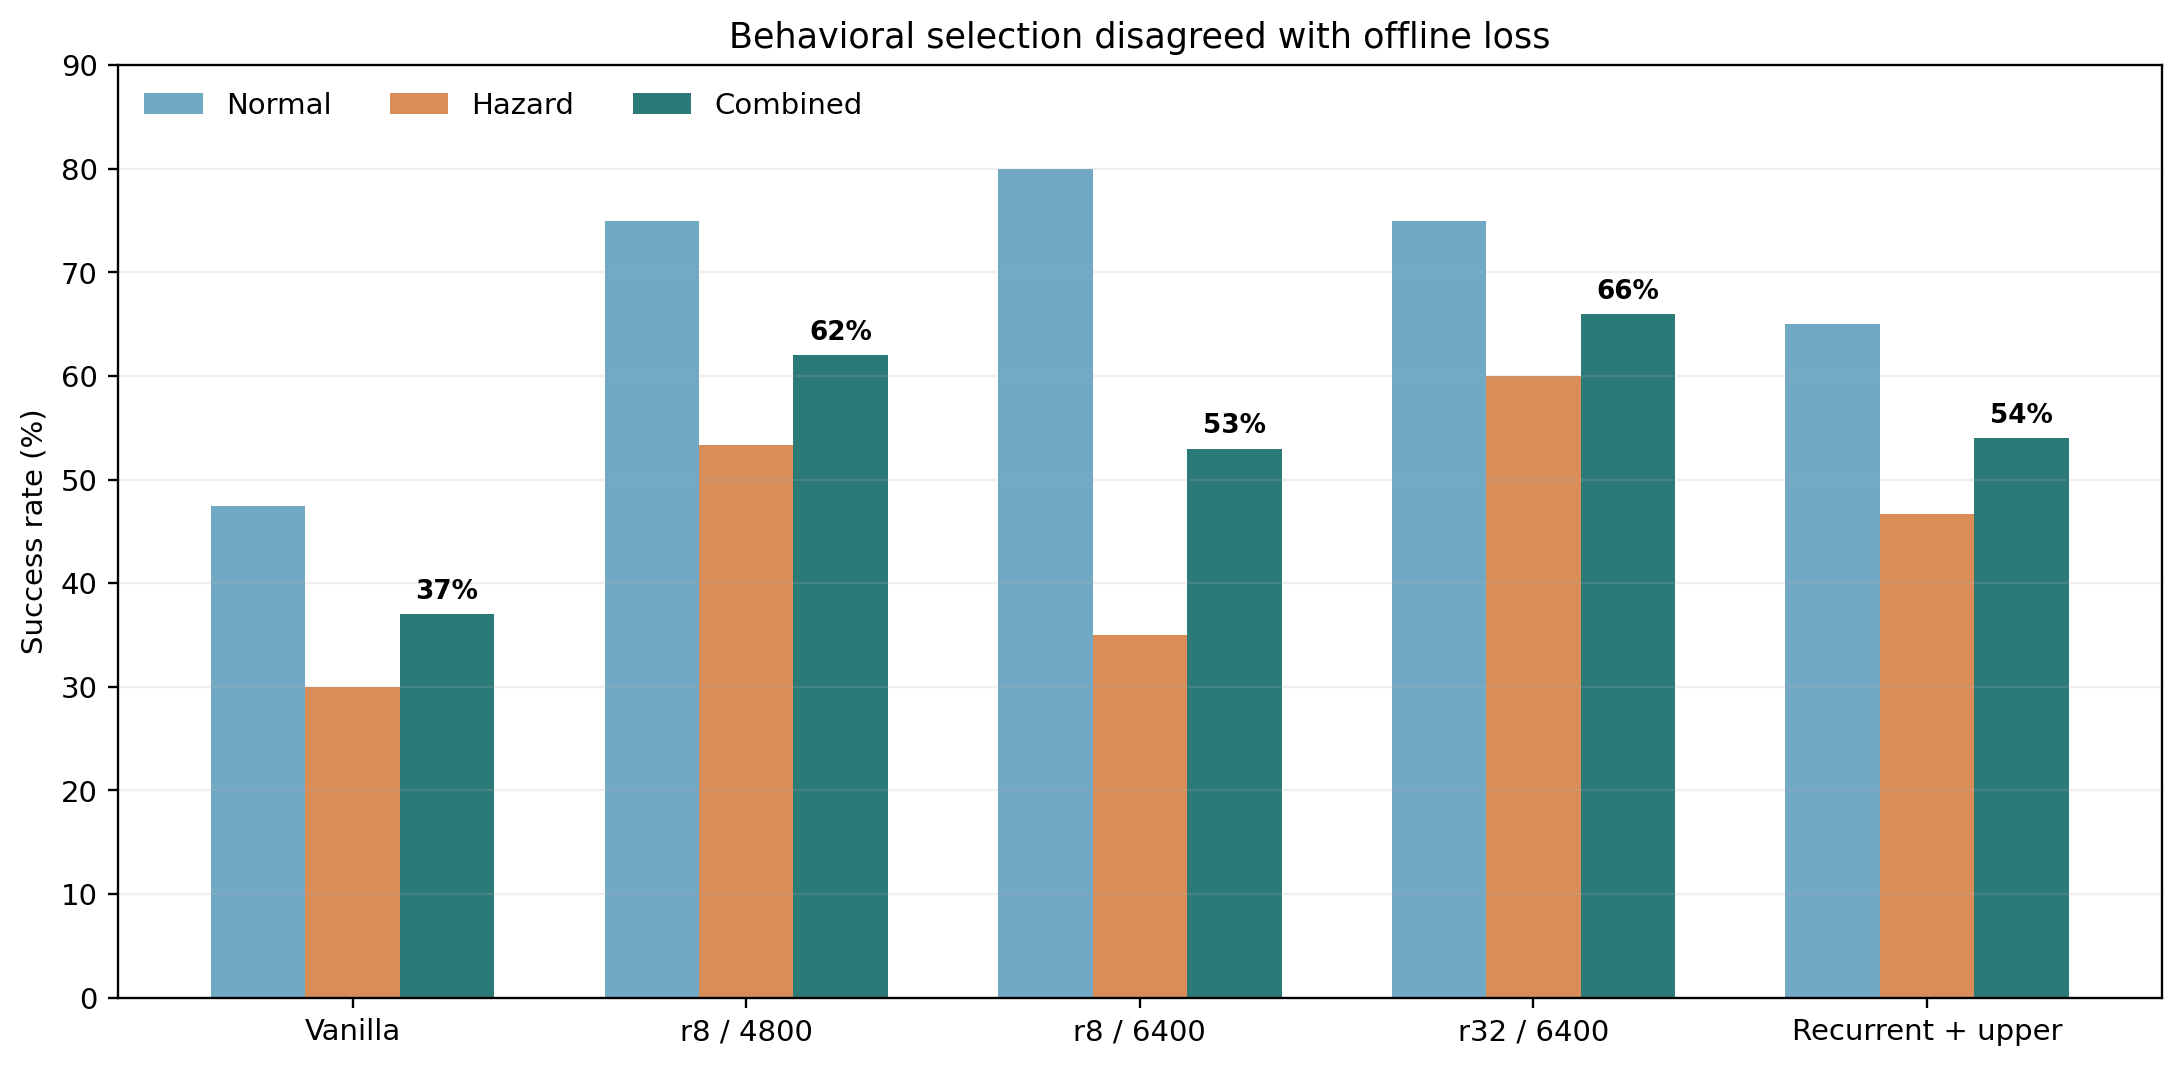
\includegraphics[width=0.86\textwidth]{figures/behavioral_screen.png}
  \caption{Paired stone-acquisition screen. Rank-32 upper LoRA at step 6400 achieved 66\% combined success versus 37\% for vanilla, despite rank-8 having the best offline validation loss.}
  \label{fig:behavioral}
\end{figure*}

\subsection{System 0 correctness was not sufficient}
The old router and old pickup controller remained the 66\% champion. Hardened pickup with the old router eliminated strict pickup-tail failures (3 to 0) but reduced success to 58\%. The new router with old pickup scored 62\%; combining both changes scored 57\% (Fig.~\ref{fig:system0}). The hardened controller returned \texttt{NEEDS\_SYSTEM1} 36 times, but the handoff did not reliably restore productive behavior.

This result generalizes beyond Minecraft: modules cannot be optimized independently when handoff semantics change the state distribution seen by downstream controllers. Verification prevented false local success, but did not guarantee useful recovery.

\begin{figure*}[t]
  \centering
  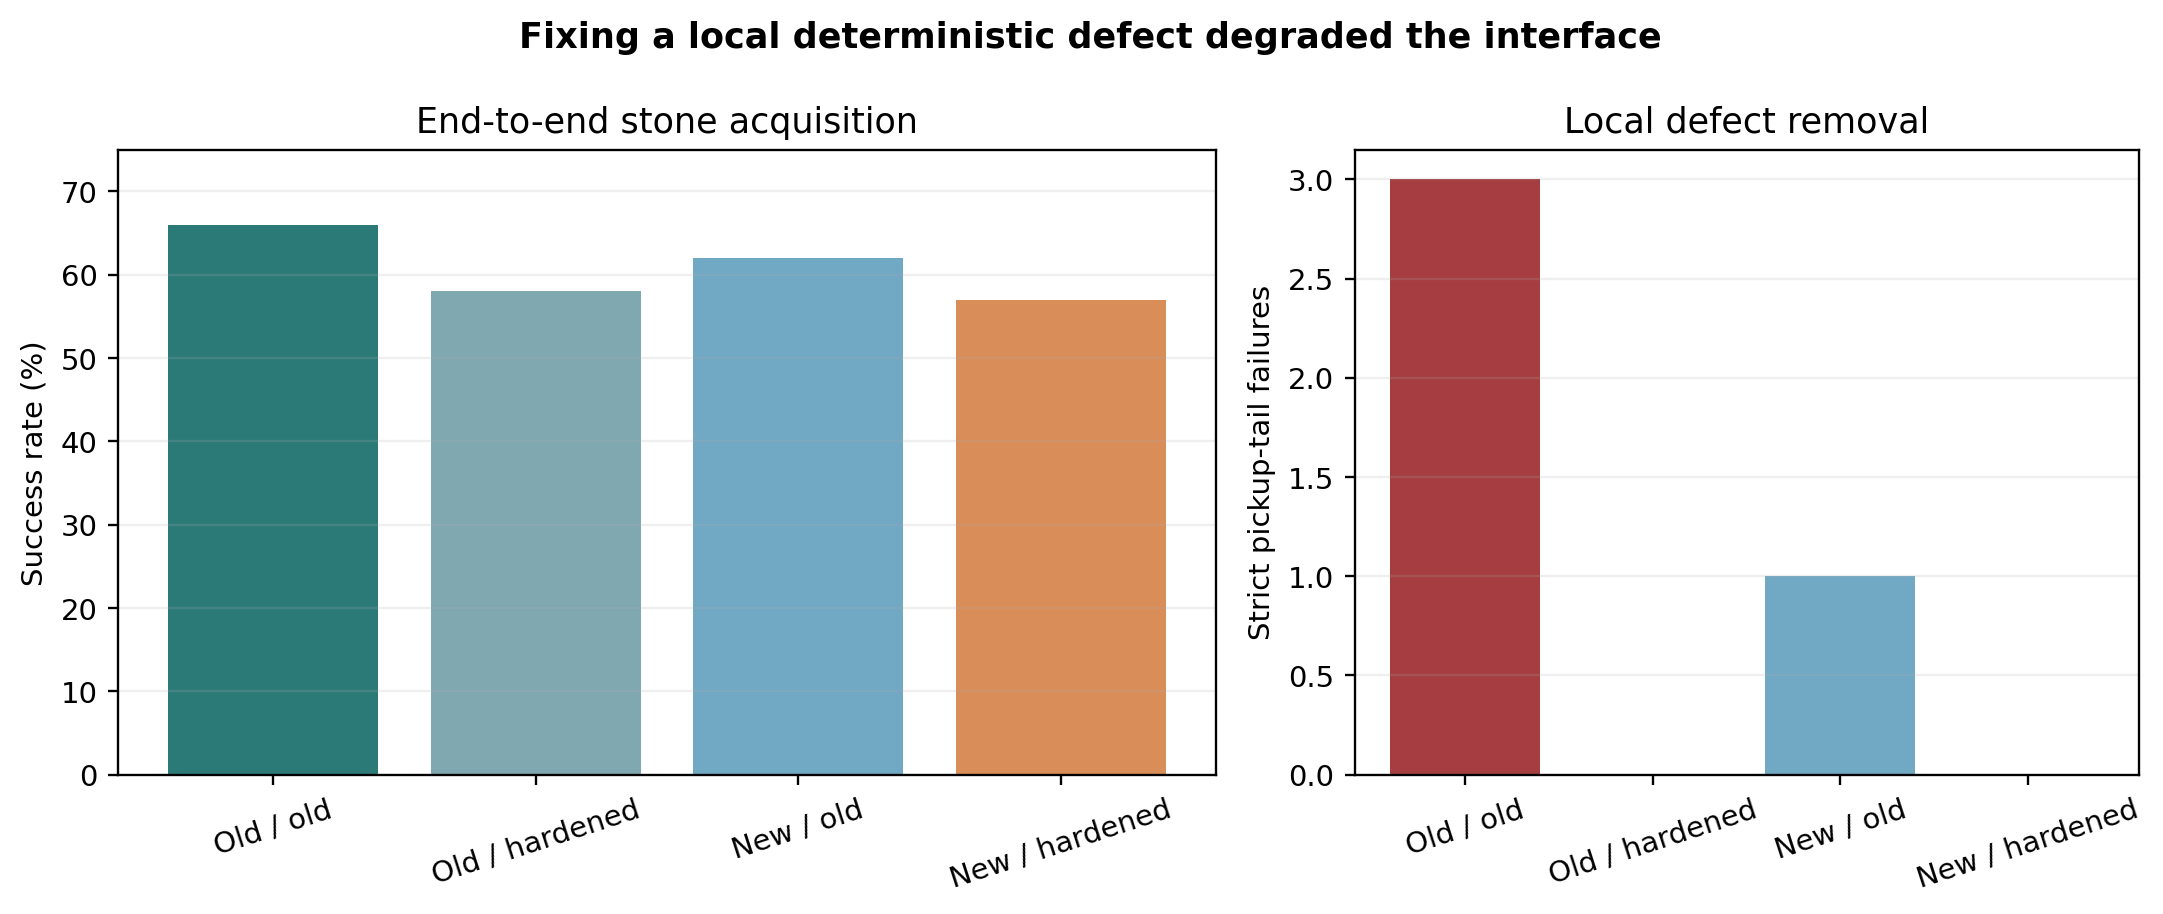
\includegraphics[width=0.85\textwidth]{figures/system0_boundary.png}
  \caption{Hardened pickup eliminated strict pickup-tail failures but reduced end-to-end success. Router changes also failed to improve the champion.}
  \label{fig:system0}
\end{figure*}

\subsection{Micro-benchmarks localized the System 1 deficit}
The asymmetry was sharp (Table~\ref{tab:micro}). Exiting water succeeded in 49/50 episodes, but climbing a shore succeeded in 5/50, escaping a hole in 4/50, avoiding water in 2/50, and both trap avoidance and camera recovery in 0/50. Gemini criticized all 50 camera failures as bad camera orientation and all 50 trap failures as mining into a trap; exact environment predicates independently confirmed the failures.

\begin{table}[t]
\centering
\caption{Controlled recovery success before and after PPO.}
\label{tab:micro}
\scriptsize
\begin{tabular}{@{}lrr@{}}
\hline
Capability & r32/6400 & PPO \\
\hline
Exit water & 98\% & 92\% \\
Reacquire stone & 30\% & 34\% \\
Climb shore & 10\% & 10\% \\
Escape hole & 8\% & 8\% \\
Avoid water & 4\% & 10\% \\
Avoid digging trap & 0\% & 0\% \\
Recover camera & 0\% & 0\% \\
\hline
\end{tabular}
\end{table}

\begin{figure*}[t]
  \centering
  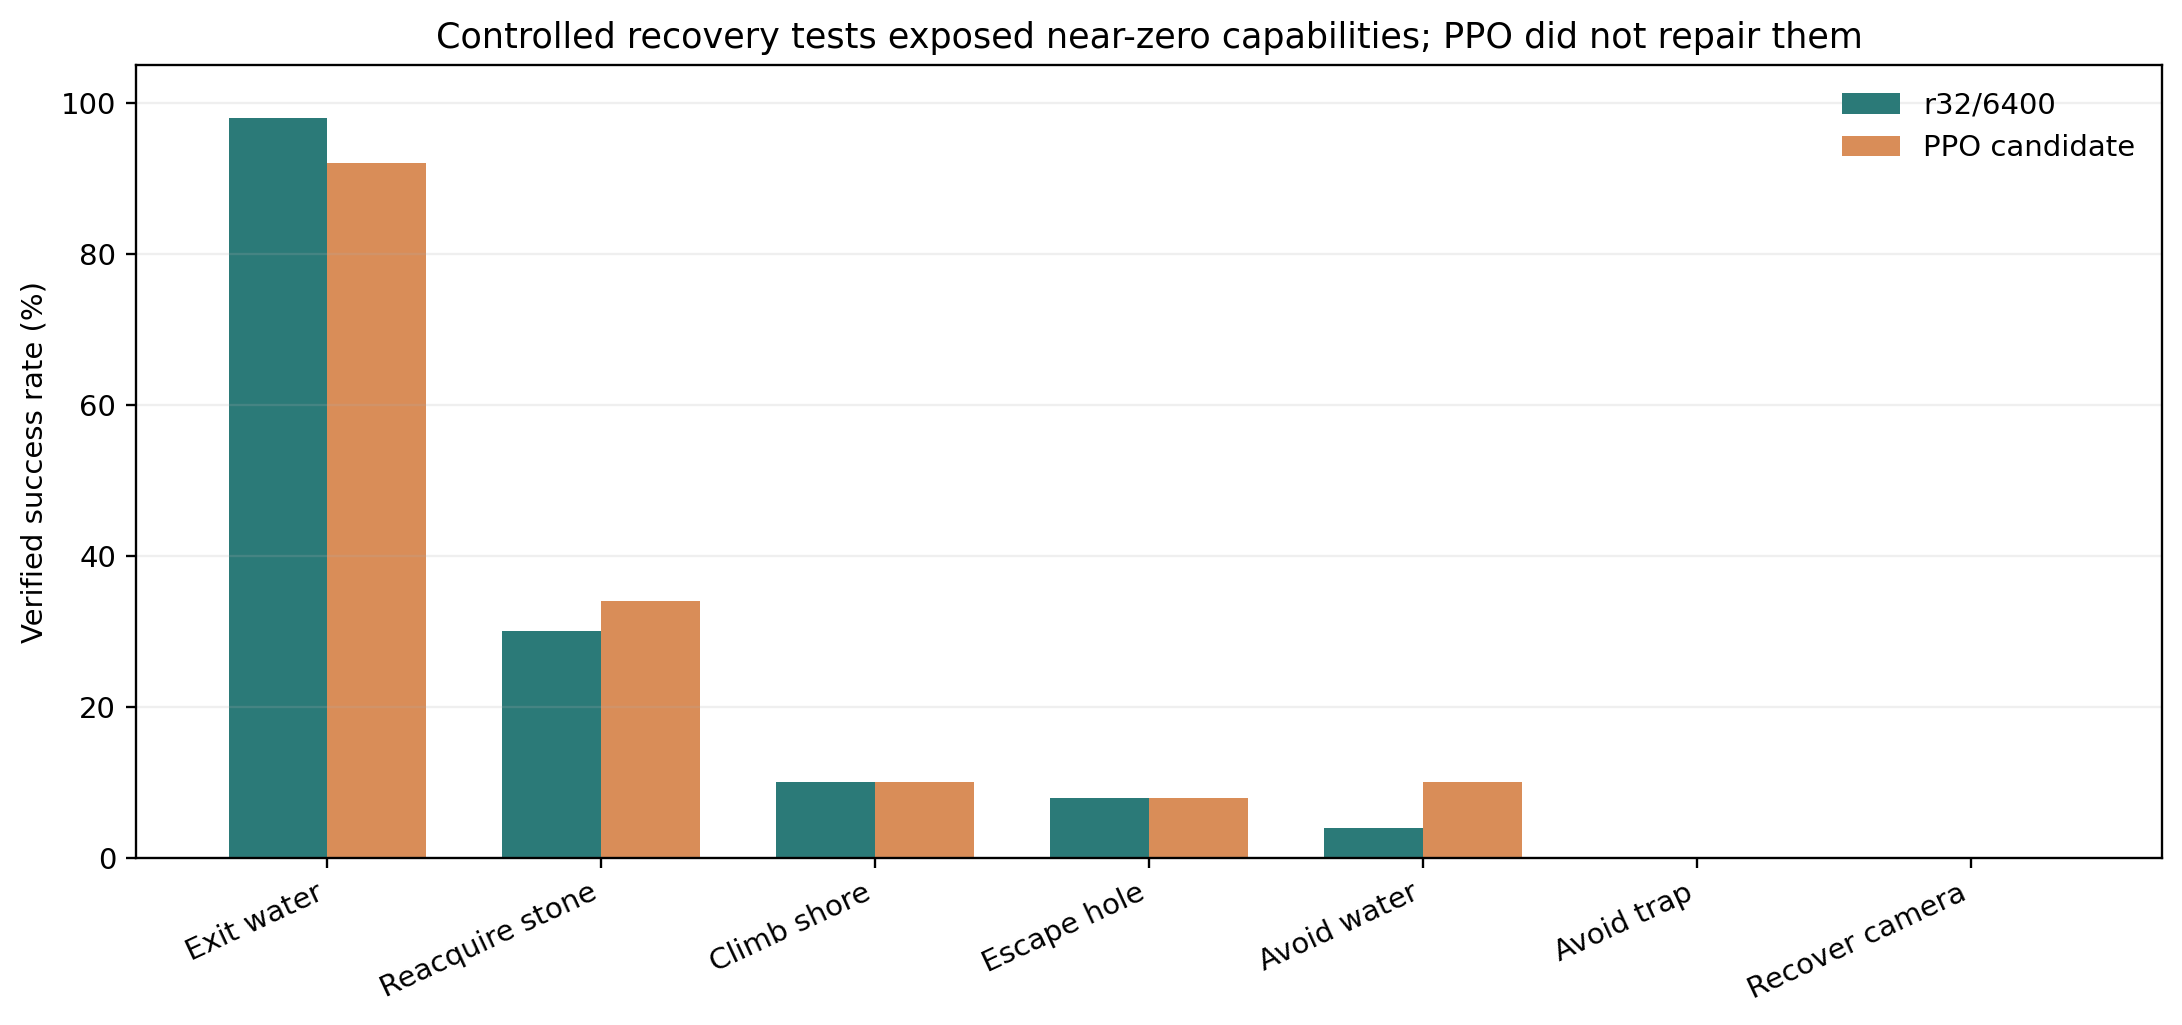
\includegraphics[width=0.88\textwidth]{figures/micro_and_ppo.png}
  \caption{Exact controlled recovery success. Exit-water was nearly solved; camera recovery and trap avoidance remained at zero. PPO did not repair these capabilities.}
  \label{fig:micro}
\end{figure*}

\subsection{Targeted PPO failed the promotion gate}
The best development checkpoint improved weak-task mean success from 13.3\% to 20.0\% and normal-stone success from 70\% to 75\%. That signal did not survive frozen evaluation. Reacquisition moved from 30\% to 34\%, camera recovery and trap avoidance remained at 0\%, and exit-water fell from 98\% to 92\%.

End-to-end stone success fell from 66\% to 54\% (difference $-12$ points; paired bootstrap 95\% CI $[-23,-1]$). Hazard success fell by 18.3 points with exact McNemar $p=0.0347$. The PPO candidate was correctly rejected.

\begin{figure*}[t]
  \centering
  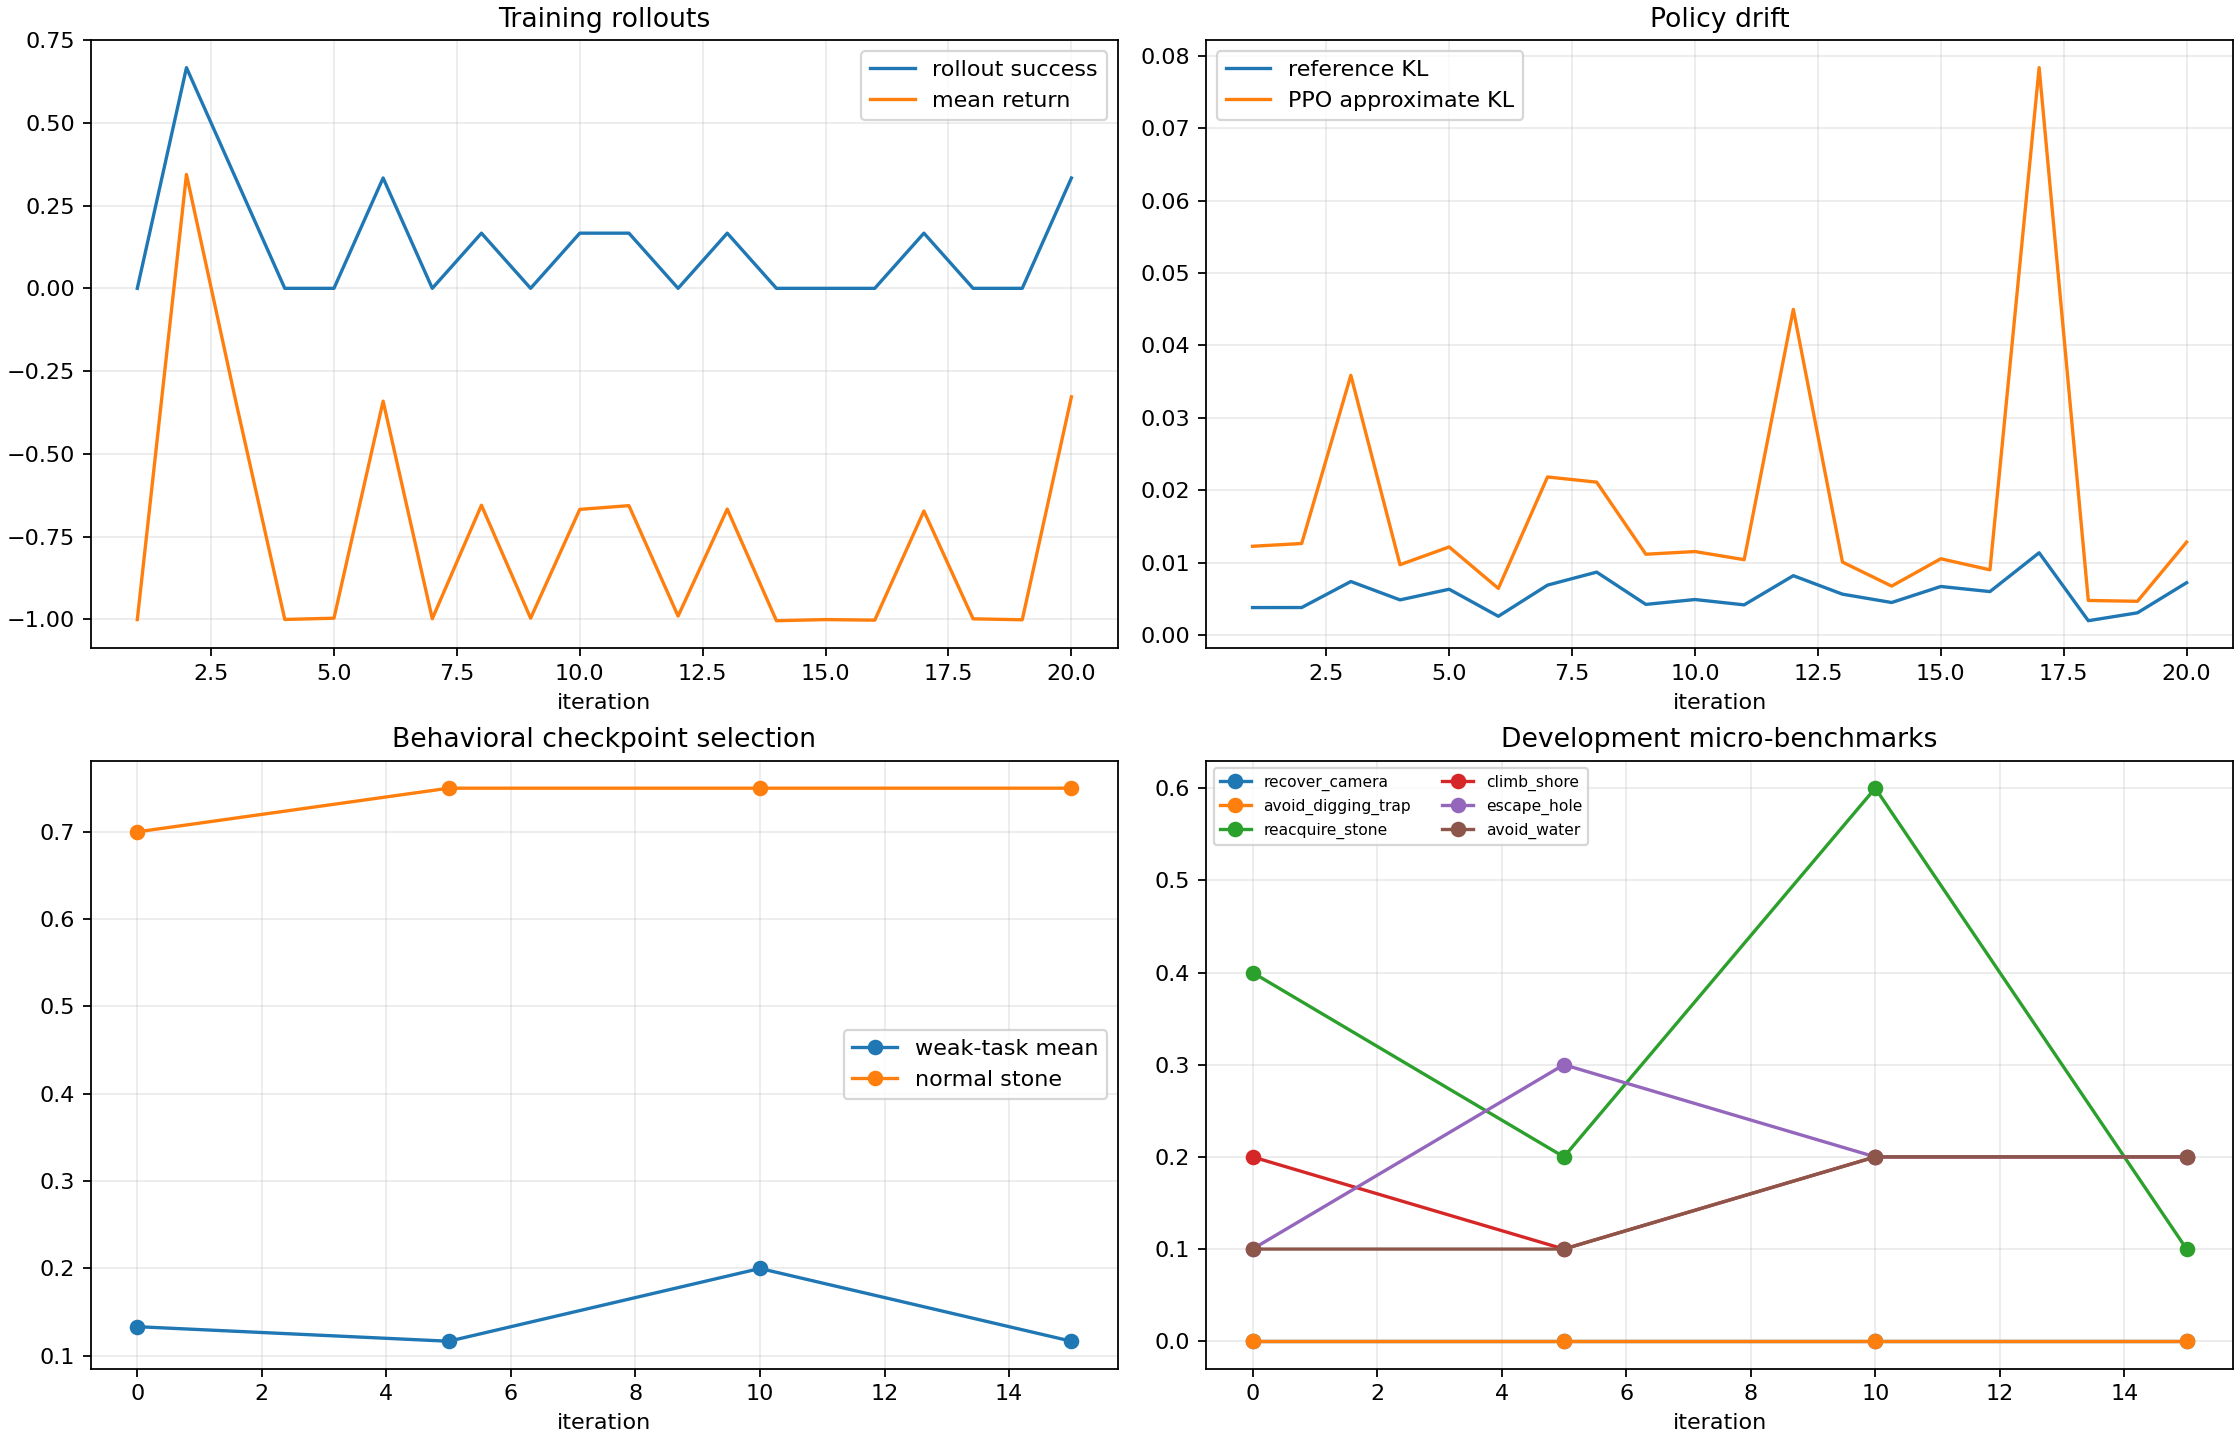
\includegraphics[width=0.92\textwidth]{figures/ppo_training_curves.png}
  \caption{PPO diagnostics. Development reacquisition briefly improved, but most weak tasks remained flat and final end-to-end hazard performance regressed.}
  \label{fig:ppo}
\end{figure*}

\subsection{Long-horizon viability: no system built an iron pickaxe}
Neither learned arm reached smelted iron (Table~\ref{tab:iron}). The scripted no-System-2 controller obtained logs in all 24 runs and three cobblestone in 13, but never produced a stone pickaxe, exposing a hierarchy/controller defect. Live System~2 clearly progressed farther: both Gemini arms produced stone pickaxes and furnaces. Yet the specialist did not improve composition. Full reached a stone pickaxe in 68.2\% and a furnace in 50.0\%, while No Specialist reached 75.0\% and 70.8\% on their respective valid denominators. Full reached three raw iron twice versus once for No Specialist, but these counts are too small for superiority claims. No arm produced an iron ingot.

The final two Full episodes were not run after prepaid API credit was exhausted. Since all observed collapse occurred before smelting and no arm had any final success, the missing episodes cannot rescue the viability claim; they do prevent a formal 24-seed paired comparison of intermediate milestones.

\begin{table}[t]
\centering
\caption{Fresh-world iron-pickaxe milestones.}
\label{tab:iron}
\scriptsize
\begin{tabular}{@{}lrrrrr@{}}
\hline
Arm & Valid & Stone pick & Furnace & Raw iron & Iron pick \\
\hline
Full & 22 & 15 & 11 & 2 & 0 \\
No specialist & 24 & 18 & 17 & 1 & 0 \\
No System 2 & 24 & 0 & 0 & 0 & 0 \\
\hline
\end{tabular}
\end{table}

\begin{figure*}[t]
  \centering
  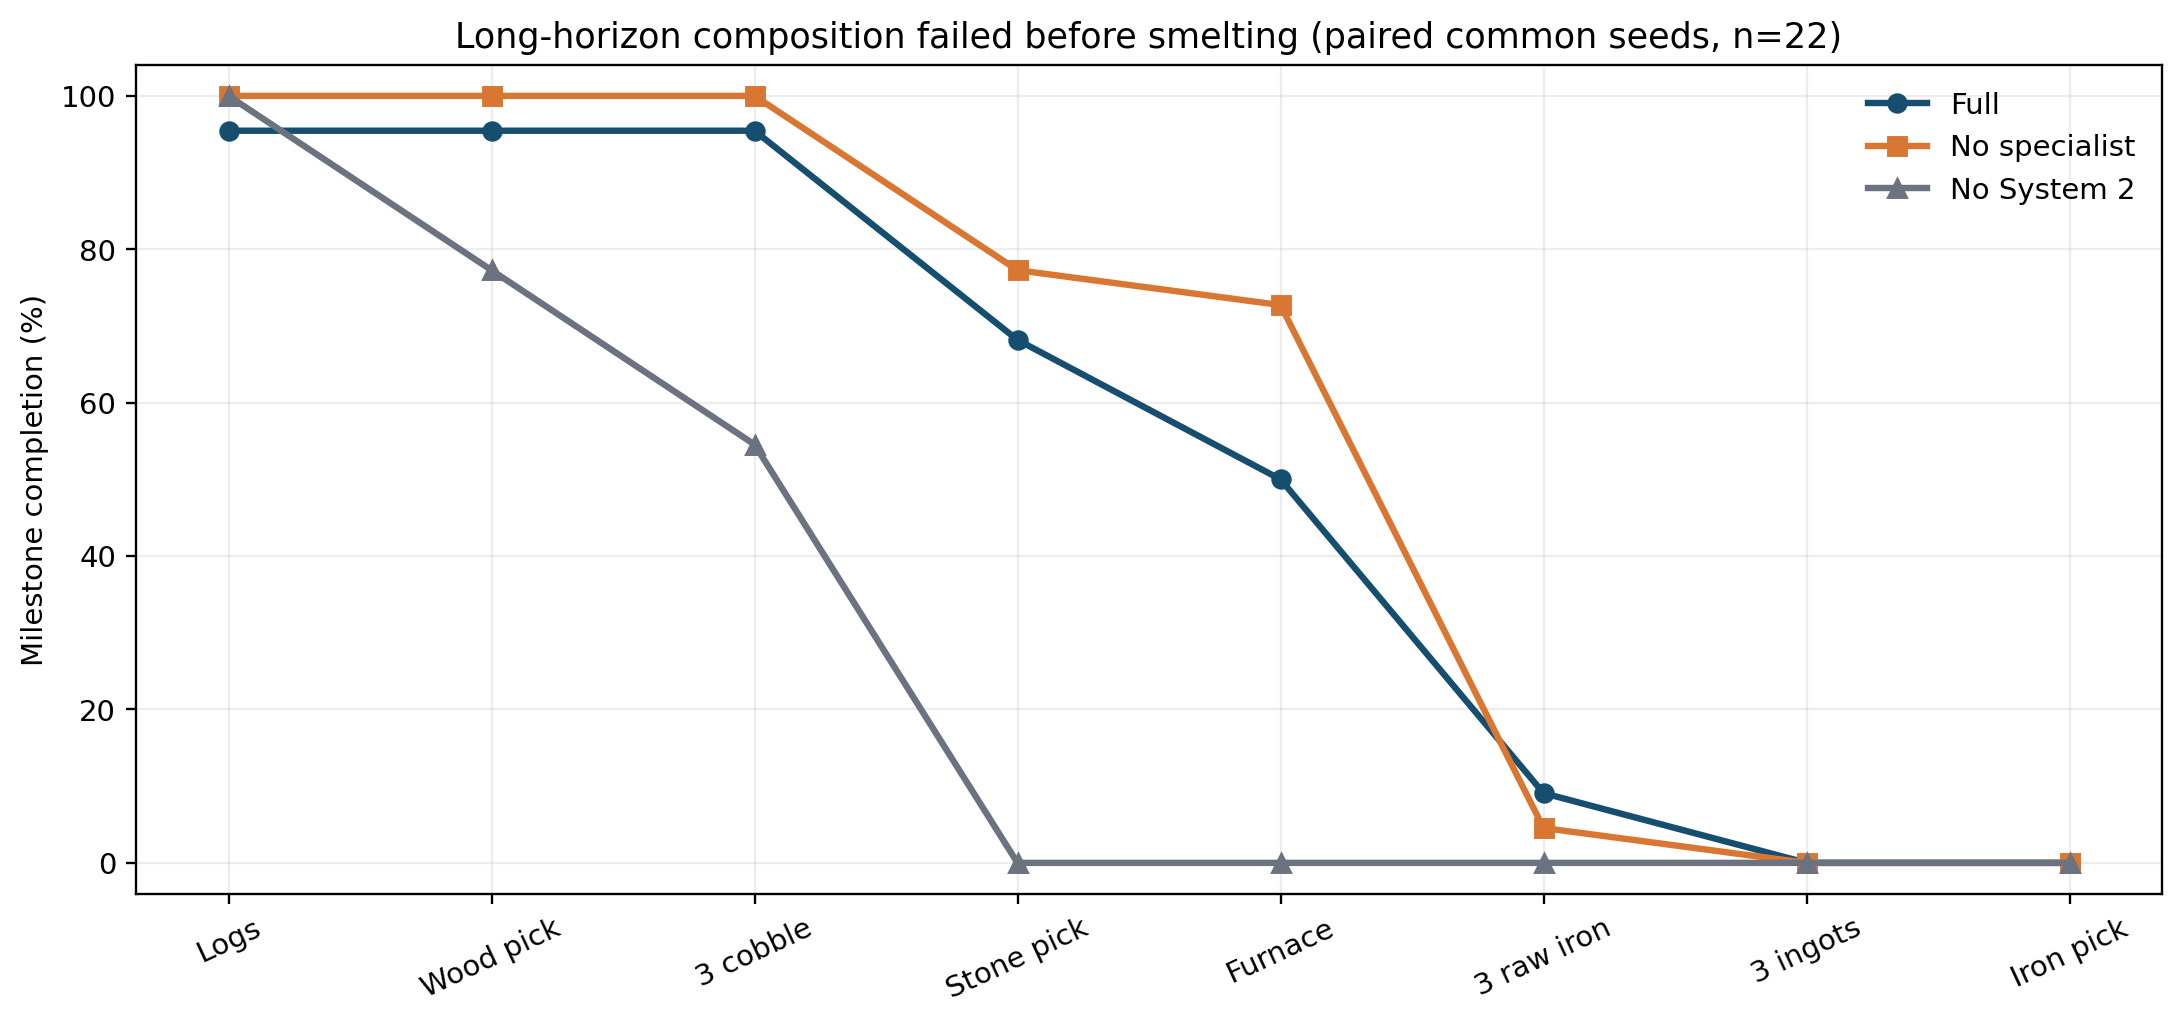
\includegraphics[width=0.88\textwidth]{figures/iron_milestones.png}
  \caption{Milestone completion on the 22 seeds common to all three arms. The full architecture and no-specialist control progressed farther than the fixed hierarchy, but neither reached smelted iron.}
  \label{fig:iron}
\end{figure*}

\begin{figure*}[t]
  \centering
  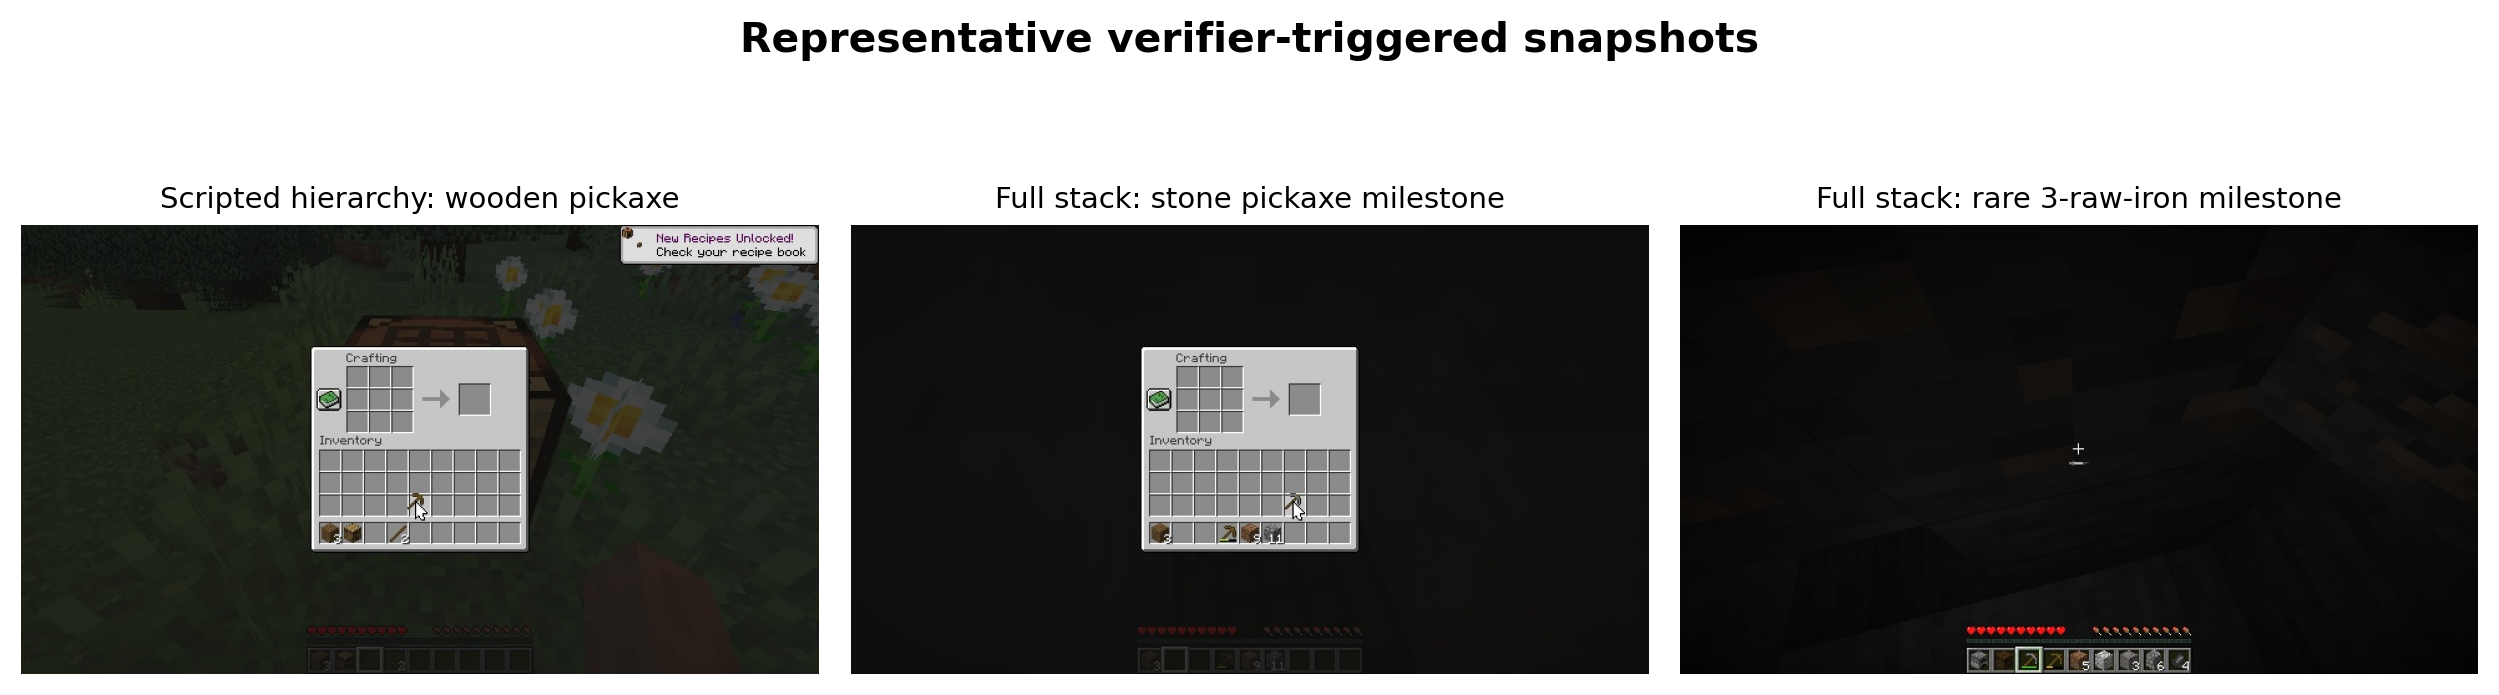
\includegraphics[width=0.94\textwidth]{figures/milestone_snapshots.png}
  \caption{Representative verifier-triggered snapshots. The architecture repeatedly established early tools and occasionally reached raw iron, but never produced three iron ingots.}
  \label{fig:snapshots}
\end{figure*}

\section{Failure Ownership}
System~1 was the dominant bottleneck in controlled recovery, but it was not the only one. System~2 advanced beyond the fixed controller, yet repeatedly selected infeasible crafting or recovery actions. System~0 removed deterministic variance only when its termination contract matched a state from which System~1 could resume. The router determined whether uncertainty was contained or amplified.

\begin{table*}[t]
\centering
\caption{Residual failure ownership.}
\label{tab:ownership}
\small
\begin{tabular}{@{}p{0.12\textwidth}p{0.35\textwidth}p{0.46\textwidth}@{}}
\hline
Owner & Supported responsibility & Observed residual failure \\
\hline
System 0 & Crafting, equipment, station use, known-target mechanics & Local correctness did not ensure recoverable handoffs; the fixed hierarchy stalled before stone-pickaxe completion. \\
System 1 & Search, approach, terrain, camera, target reacquisition & 0\% camera recovery, 0\% trap avoidance, 8\% hole escape, and 10\% shore climb. \\
System 2 & State tracking, objective choice, replanning & Progressed beyond the script, but made repeated infeasible choices; long episodes averaged roughly 28--29 replans. \\
Interface & Preserve context and switch at stable boundaries & Strict ambiguity handoffs and fewer transitions still degraded end-to-end success. \\
\hline
\end{tabular}
\end{table*}

\section{Discussion}
\paragraph{The narrow result is real.}
A rank-32 LoRA improved a difficult paired benchmark by 29 points with strong statistical evidence. This supports interchangeable task specialists as a practical way to adapt a large motor prior without retraining a foundation policy.

\paragraph{The broad thesis is not supported.}
The specialist gain did not improve the long-horizon hierarchy, and the full architecture achieved zero final successes. Relative to published VPT or STEVE-1 results, this study is neither a model-scale comparison nor a reproduction: tasks, budgets, prompts, checkpoints, and evaluation distributions differ. It would be incorrect to claim superiority.

\paragraph{Modularity created measurable interface debt.}
Eliminating strict pickup-tail failures made the agent worse because ambiguity triggered handoffs that the learned controller could not exploit. The correct optimization unit spans option termination, state representation, router policy, and resumed controller context.

\paragraph{Behavioral selection must dominate proxy losses.}
Rank-8 won offline; rank-32 won online. PPO reward and development micro-tests also selected a checkpoint that regressed on the paired hazard benchmark. Small frozen behavioral gates are necessary throughout training.

\paragraph{LLM spending did not purchase motor competence.}
Gemini was useful for planning and failure taxonomy, but repeated calls were expensive and did not solve camera, terrain, or target reacquisition. Exact verifiers were cheaper and more reliable for reward and completion. An economical design should invoke System~2 only on meaningful state changes, cache plans, and sample trajectory critics sparsely.

\section{Limitations}
\begin{itemize}
  \item This is a single-project engineering study, not a standardized MineRL leaderboard submission.
  \item The 1,000-episode stage-0 distribution and 100-episode behavioral screen differ; their absolute rates are not directly comparable.
  \item The final Full arm contains 22 rather than 24 valid episodes.
  \item Gemini critiques are correlated observations, not independent ground truth; environment predicates control quantitative claims.
  \item The long-horizon test exposed crafting and fixed-hierarchy defects, so it mixes component quality with integration quality.
  \item We make no claims of human-level play, general Minecraft competence, or superiority to published VPT, STEVE-1, Voyager~\cite{voyager}, or MineStudio baselines.
\end{itemize}

\section{Conclusion}
The System~0/1/2 framing was useful, but the current agent is not a viable long-horizon Minecraft system. The project demonstrated that targeted BC can create a materially stronger specialist and that deterministic options can compress exact mechanics. It also established three negative results: module-local correctness can reduce system success, targeted PPO can erase a good behavioral prior, and live frontier-model planning cannot overcome a weak recovery interface. The defensible conclusion is that \emph{composition must be trained and evaluated as its own capability}. Without that, the architecture remains an insightful diagnostic scaffold around an insufficient body.

Given zero iron-pickaxe completions and the high API cost of final evaluation, stopping additional patching was rational. A future restart should require a cheaper deterministic integration harness, explicit option-to-policy recovery state, and a pre-registered promotion gate on complete long-horizon milestones.

\section{Reproducibility and Artifact Disposition}
The retained DGX state contains the official STEVE-1 checkpoint, the immutable rank-32/6400 specialist, compact JSON reports and result rows, representative images, SHA-256 manifests, and source code. Raw rollouts, smoke outputs, superseded architectures, failed PPO candidates, and unused GROOT/ROCKET/VPT checkpoints were removed after the archive and champion were hash-verified. The cleanup released approximately 216~GB from the MineStudio project tree. The paper bundle contains the reports used to generate every table and chart.

\begin{thebibliography}{9}
\bibitem{vpt} B. Baker et al., ``Video PreTraining (VPT): Learning to Act by Watching Unlabeled Online Videos,'' \emph{NeurIPS}, 2022. \url{https://arxiv.org/abs/2206.11795}
\bibitem{steve} S. Lifshitz, K. Paster, H. Chan, J. Ba, and S. McIlraith, ``STEVE-1: A Generative Model for Text-to-Behavior in Minecraft,'' \emph{NeurIPS}, 2023. \url{https://arxiv.org/abs/2306.00937}
\bibitem{minestudio} S. Cai et al., ``MineStudio: A Streamlined Package for Minecraft AI Agent Development,'' arXiv:2412.18293, 2024. \url{https://arxiv.org/abs/2412.18293}
\bibitem{voyager} G. Wang et al., ``Voyager: An Open-Ended Embodied Agent with Large Language Models,'' \emph{TMLR}, 2024. \url{https://arxiv.org/abs/2305.16291}
\bibitem{ppo} J. Schulman et al., ``Proximal Policy Optimization Algorithms,'' arXiv:1707.06347, 2017. \url{https://arxiv.org/abs/1707.06347}
\bibitem{lora} E. Hu et al., ``LoRA: Low-Rank Adaptation of Large Language Models,'' \emph{ICLR}, 2022. \url{https://arxiv.org/abs/2106.09685}
\end{thebibliography}

\end{document}
